\documentclass[12pt]{article}
\usepackage{amssymb}
\usepackage{graphicx} % Required for inserting images
\usepackage[paperheight=29.7cm,paperwidth=21cm]{geometry}
\usepackage{wrapfig}
\usepackage[
backend=biber,
style=apa,
]{biblatex}
\addbibresource{main.bib} %Imports bibliography file

\title{An Analysis into Exact Trigonometric Ratios and Sine of 1 degree}
\author{Gautam Bansal}
\date{February 2025}

\usepackage{setspace}
\doublespacing
\newcommand{\specialcell}[2][c]{%
  \begin{tabular}[#1]{@{}c@{}}#2\end{tabular}}
\begin{document}
\maketitle

\section{Introduction}
   
\subsection{Rationale}
 I chose this topic as I am fascinated by the way the imaginary realm of imaginary numbers can connect to the values of sine and cosine, while geometry and algebra can both be intrinsically connected by such trigonometric ratios. To analyse this connection, one of the best values for a trigonometric ratio to choose would be the sine of 1 degree. This is because even though it may seem very simple, it in fact can be found in multiple ways involving various other trigonometric ratios, along with understanding the roots of unity and complex numbers. Based on preliminary research, sin(3 degrees) has been found using angle difference formulas with sin(18) and sin(15), which were found by geometry, but finding sin(1 degree) exactly in terms of real numbers has not been done. Using De Moivre's theorem along with algebra, however, this value could be found.  

\subsection{Prior Knowledge}
To clarify how sine ratios work, why they are important, and showing a simple example of derivation of a sine ratio that will later become useful, prior knowledge is required before entering the main investigation.
\subsubsection{Trigonometric Ratios}

\textbf{Trigonometric ratios}, such as sine, cosine, and tangent, are vital in geometry, and even other realms of math and the real world.

Taking a right triangle ABC, for the angle $\angle$A we can take ratio of the side opposite to it to the hypotenuse. This would be the sine ratio of A or sin(A) and is constant based on the measure of angle A since in a triangle if two angles are fixed, then the ratio of sides must be fixed. We can see opposite, adjacent, and hypotenuse visually in Figure \ref{fig:OHA}.

\begin{figure}[h]
    \centering
    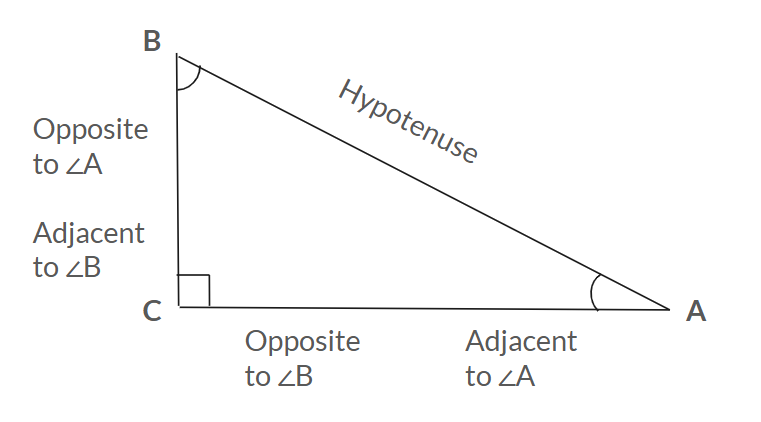
\includegraphics[width=0.5\linewidth]{OppAdjHyp.png}
    \caption{Opposite, Adjacent, and Hypotenuse in a Triangle}
    \label{fig:OHA}
\end{figure}

There are similar ratios for cosine and tangent as mentioned below. 
\begin{center}
    $\sin$ = $\frac{opposite}{hypotenuse}$,  $\cos$ = $\frac{adjacent}{hypotenuse}$, $\tan$ = $\frac{opposite}{adjacent}$
\end{center}

These ratios are important throughout mathematics, as their functions can in fact be found everywhere - from electromagnetic waves to pendulum motion! In Figure \ref{fig:sct}, the graphs of all three functions are shown. As this paper focuses on sine, one important property of sin(x), that is clear in the shown graph, is that it approaches x for small values of x. 

\begin{figure}[h]
    \centering
    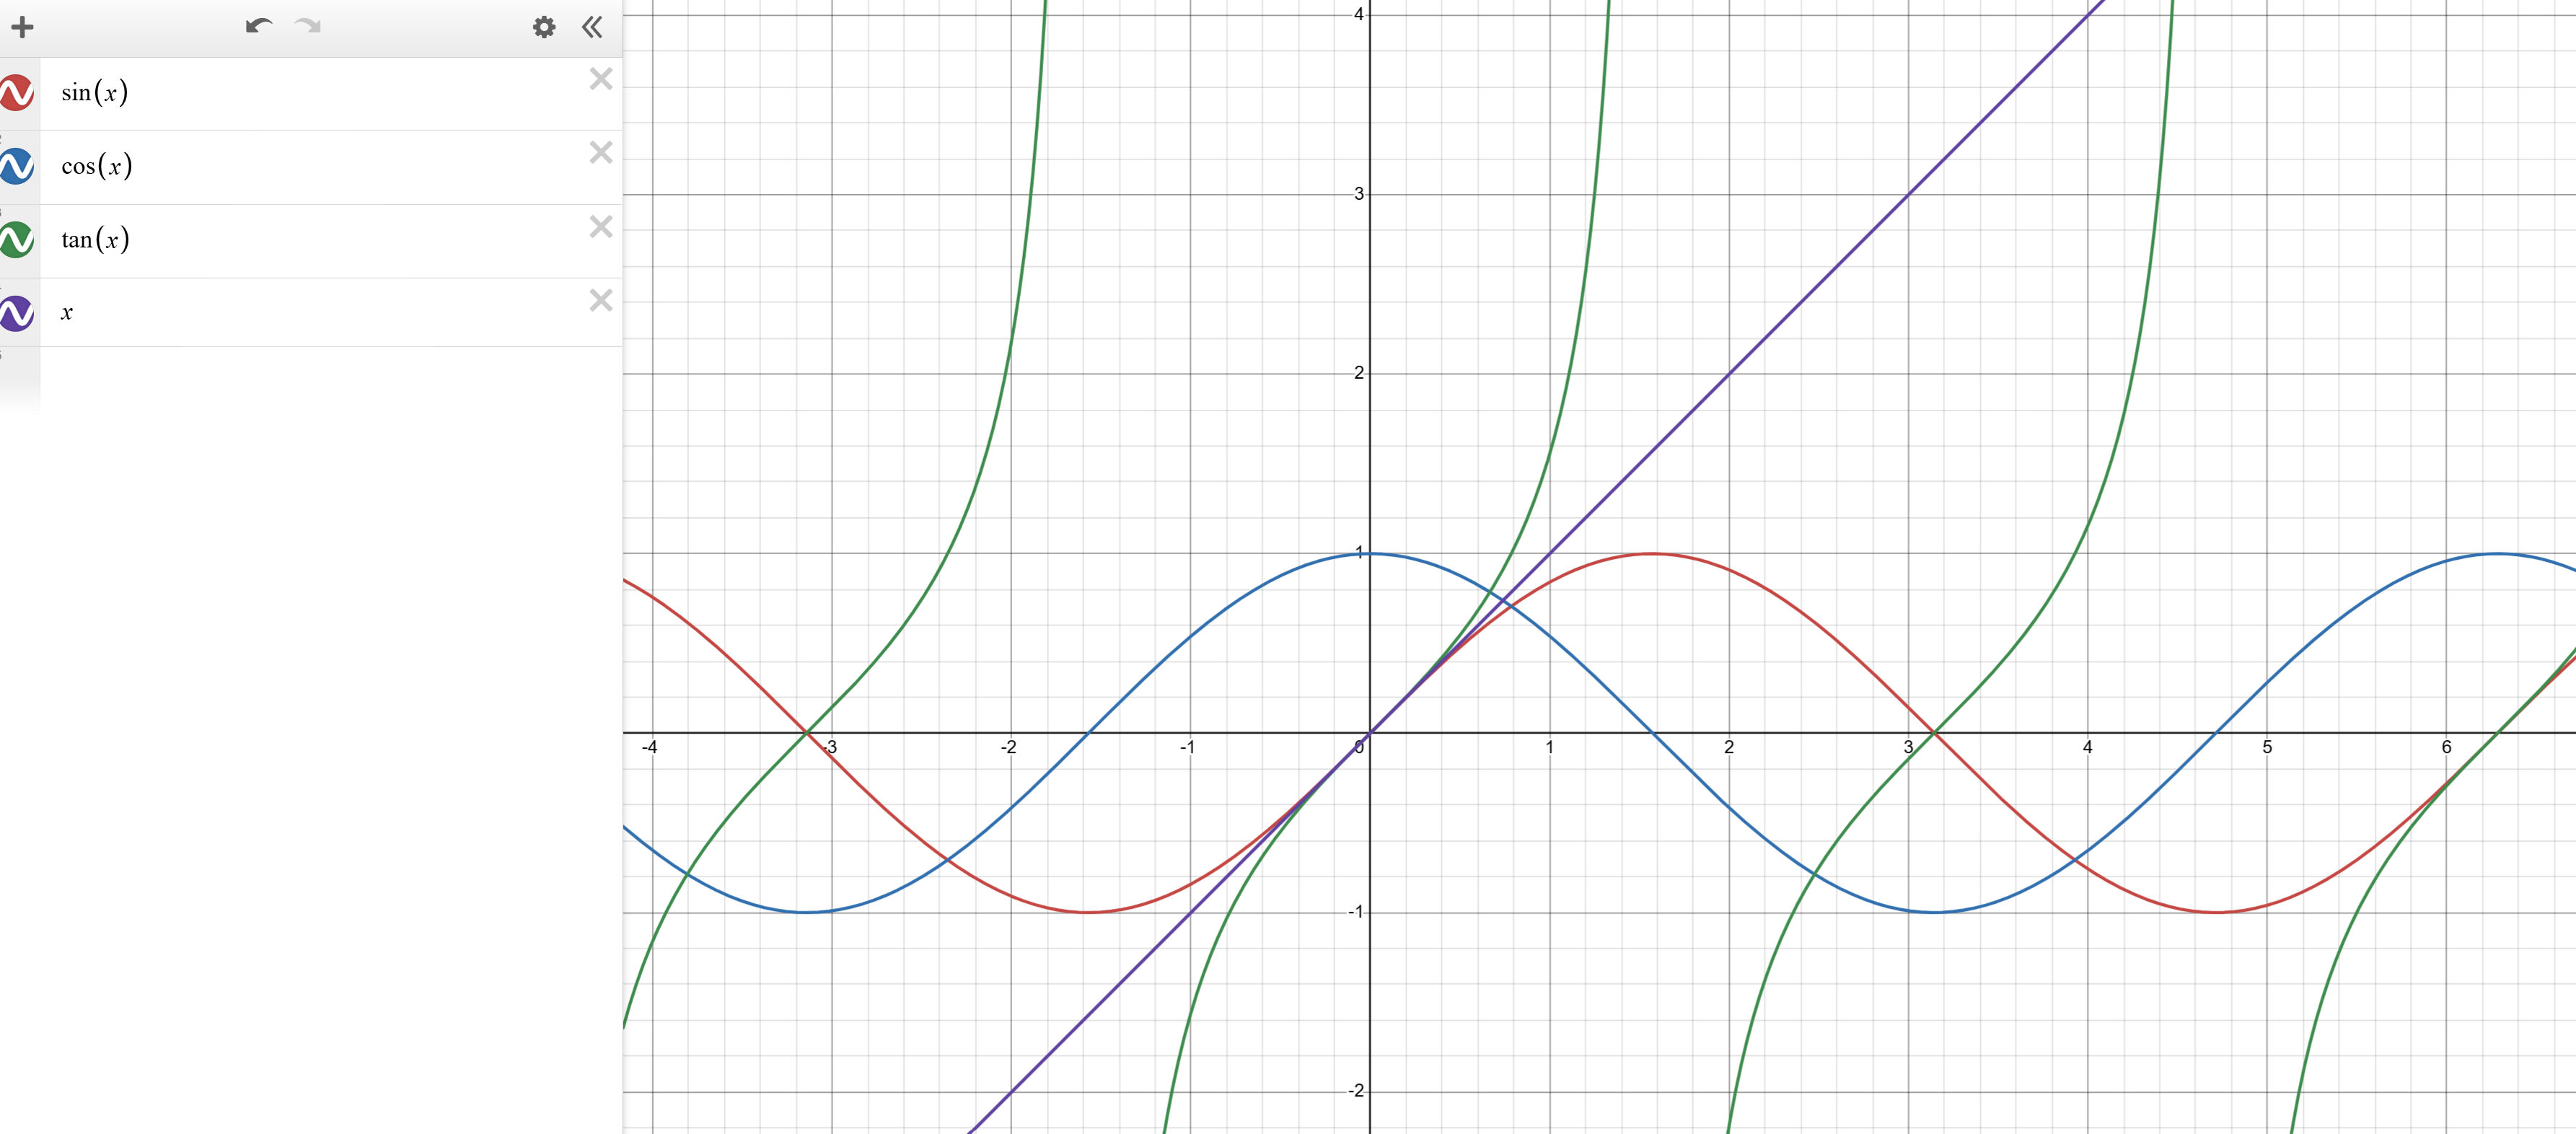
\includegraphics[width=0.8\linewidth]{sincostangraphs.png}
    \caption{The Graphs of Sin(x), Cos(x), and Tan(x)}
    \label{fig:sct}
\end{figure}            

\subsubsection{Derivation of sin(30) with Geometry}
The derivation of sin(30) through basic geometric rules is important prior knowledge to finding sin(15).

\begin{figure}[h]
    \centering
    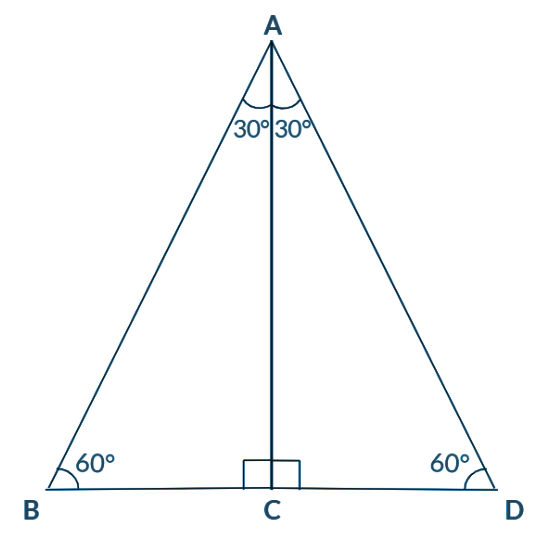
\includegraphics[width=0.4\linewidth]{306090triangle.png}
    \caption{Equilateral Triangle Used for Deriving Sin(30)}
    \label{fig:30}
\end{figure}

Let us take an equilateral triangle ABD, and split it using a median from A to BD, forming segment AC, as shown in Figure \ref{fig:30}.


As it is an equilateral triangle and the angles must sum to 180 degrees, we know that each interior angle of the equilaterial triangle is 60$^{\circ}$.

Since it is a median, BC must equal CD, and the sides of an equilateral triangle are equal (AB=AD), making ABC congruent to ADC by Side-Angle-Side congruency.

As they are congruent, and we know $\measuredangle$BCA + $\measuredangle$ACD = 180, meaning each of them are 90$^{\circ}$, and by angle sum theorem, $\measuredangle$BAC and $\measuredangle$CAD must each be 30$^{\circ}$.

As BC must be half of AB since the sides of the triangle are equal and the median cuts BD in half, this automatically means sin(30$^{\circ}$) is 1 divided by 2, or 0.5. Similarly, using Pythagoras Theorem, AC = $\sqrt{3}$ times BC, resulting in the value of sin(60$^{\circ}$) being $\frac{\sqrt{3}}{2}$.

This is essentially one example of the derivation of a sine ratio, but as we will see, deriving it for specific angles such as sin(1$^{\circ}$) is not as simple.

\subsection{Aim}
As such, the aim of this analysis is to explore how the exact value of sin(1$^{\circ}$) can be derived, with various methods. The advantages of these methods will be looked at, and the connections between complex numbers, calculus, and more to trigonometric ratios will be found.

\subsection{Methodology}
Three methods of finding the value of sin(1 degree) will be analysed, ranging across algebra and geometry, with some calculus. From Cardano's formula to the Taylor series, all types of methods will be understood and analysed, with both geometric and algebraic viewpoints. The first method involves approximating using calculus and the Taylor series, along with derivation and usage of a simple rational approximation that yields the mathematician Bhaskara's approximation for sine. The second method finds sin(18) and sin(15) with geometry, followed by using angle difference formula and then De Moivre's to yield sin(1). Finally, for the third method, sin(1) will be found with the unit circle and roots of unity.

This investigation will comprehensively look at multiple methods of sine approximation and evaluation together, and will also allow for better understanding of the effectiveness of these methods.

\section{Method 1: Approximating}
The first method to begin with is to look at two common ways of approximating sin(1) without a complete derivation. These are based off of a power series followed by a rational approximation.

\subsection{Taylor Series Approximation (Infinite Sum)}
Let us first look at the Taylor series approximation of sines. To understand the Taylor series approximation, we can use this formula provided by Brilliant.org:
\[
f(x) = f(a) + \frac{ f'(a)}{1!} (x - a) + \frac{f''(a)}{2!} (x - a)^2 + \frac{f^{(3)}(a)}{3!} (x - a)^3\cdots
\]
This formula is a method of approximating any function. By using derivatives up to the $\textit{n}$th derivative of a function, one can develop a polynomial with this formula that approximates that function. For sin(x) specifically, we can take this formula with just the first derivative (until 2nd term), for a=0, to yield $t(x)=x$. This is a fairly accurate approximation for low values of x, such as 1 degree (0.017453 rad). Note that due for a=0, as sin(0) = 0, only the even (2nd, 4th, etc.) terms from the Taylor series formula are needed, as all the odd terms result in 0. As such, we may take approximations from the Taylor series as shown in the table below, where correct digits are underlined:\\
\begin{table}[h]
    \centering
    \begin{tabular}{|c|c|c|}
        \hline
        \vtop{\hbox{\strut \textbf{Until \textit{n}th term of}}\hbox{\strut \textbf{sin(x)'s Taylor series}}} & \textbf{Series for sin(x) with a=0}& \textbf{Result for sin(1$^{\circ}$)}\\ \hline
        n = 1& $\rule[-1em]{0pt}{1.5em}\rule{0pt}{1.5em}x$& \underline{0.01745}32925199433\\ \hline
        n = 2& $\rule[-1em]{0pt}{1.5em}\rule{0pt}{1.5em}x-\frac{x^{3}}{6}$& \underline{0.0174524064}237876\\ \hline
        n = 3& $\rule[-1em]{0pt}{1.5em}\rule{0pt}{1.5em}x-\frac{x^{3}}{6}+\frac{x^{5}}{120}$& \underline{0.017452406437283}6\\ \hline
         n = 4& $\rule[-1em]{0pt}{1.5em}\rule{0pt}{1.5em}x-\frac{x^{3}}{6}+\frac{x^{5}}{120}-\frac{x^{7}}{5040}$& \underline{0.0174524064372835}\\\hline
    \end{tabular}
    \caption{Taylor Series Approximations for sin(1$^{\circ}$)}
    \label{tab:placeholder}
\end{table}

From this table, it is evident that an approximation using the only the first one or two terms of the Taylor series for sin(x) can be fairly accurate for most purposes. Further, with only 3 terms, the result is accurate to 15 decimal places, so practically, such approximations are quite useful. However, for our mathematical understanding, it is vital that we go further, as if properly calculated, a rational function based on two-degree polynomials can be found to approximate sin(x) from 0 to 2$\pi$ radians, as will be seen in Bhaskara's approximation. 

\subsection{Bhaskara's Approximation (Rational)}
Bhaskara was an Indian mathematician from the 7th century, who obtained a remarkable rational approximation of sine. The way it has been proved has never been documented, but a research paper from the University of Montana describes one possible way, which likely involved noticing features of y=sin($\theta^{\circ}$) over the domain $0\le x\le 180^{\circ}$, in order to find a second-degree polynomial approximation at first. Note that Bhaskara used degrees, and hence we may use the sin($\theta^{\circ}$) as in Figure \ref{fig:sindeg}.

\begin{figure}[h]
    \centering
    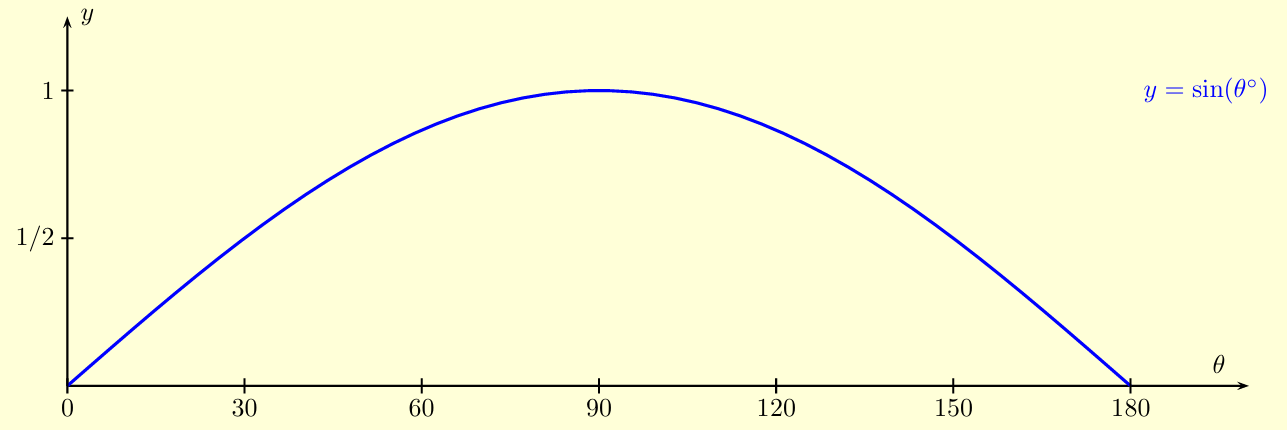
\includegraphics[width=0.75\linewidth]{sindegrees.png}
    \caption{The Graph of Sin($\theta^{\circ}$)}
    \label{fig:sindeg}
\end{figure}     

First, using simple quadratic properties, we can form a basic polynomial with zeroes at 0 degrees and 180 degrees. This would be $\theta(180-\theta)$, which in fact Bhaskara referred to as \textit{prathama} (Sanskrit for `first'), implying that this is how he began. Then, we can check for sin(90$^{\circ}$) which should equal 1, but instead it yields 8100. So, dividing this polynomial by 8100 should yield better accuracy as shown in Figure  \ref{fig:sindegA1}.

\begin{figure}[h]
    \centering
    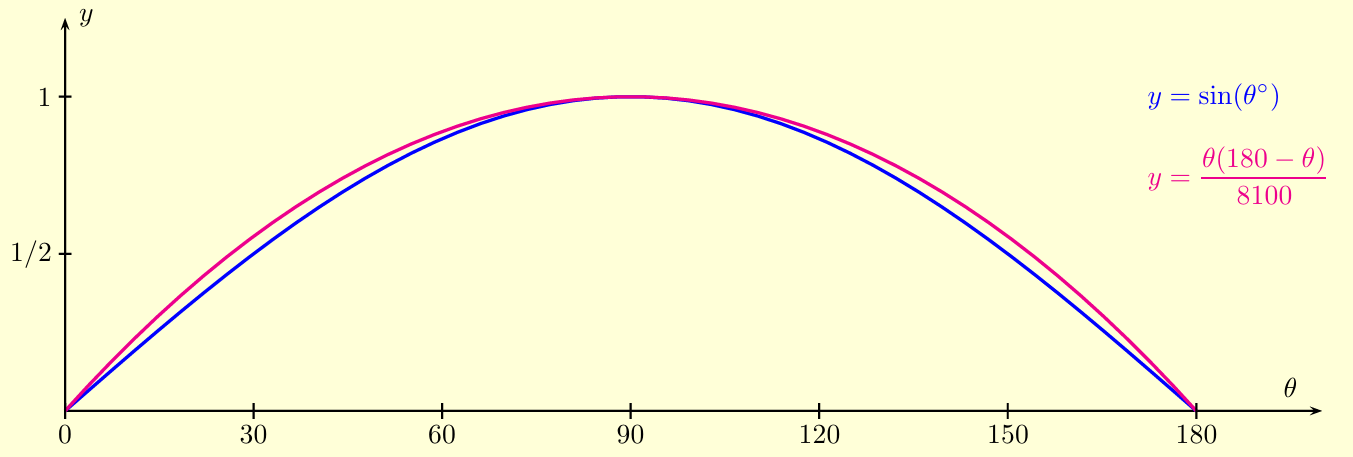
\includegraphics[width=0.75\linewidth]{sindegApprox1.png}
    \caption{The Naïve Approximation of Sin($\theta^{\circ}$)}
    \label{fig:sindegA1}
\end{figure}     

This is still far from accurate, so Bhaskara's next step would be to make sure the polynomial fits sin(30$^\circ$) = $\frac{1}{2}$. Currently, though, the result of the polynomial is $\frac{5}{9}$ for 30$^\circ$, so using the quadratic vertex form a new polynomial was made, symmetrical about 90 degrees, that yielded $\frac{10}{9}$ for 30$^\circ$. First, we have $1 +(\theta - 90)^2$, then to make it $\frac{10}{9}$ for 30$^\circ$, we can divide the second term by the constant $9(30-90)^2$ resulting in $1 +\frac{(\theta - 90)^2}{32400}$. 

The reason for this new polynomial is that dividing it from our old polynomial will give us a much better sine approximation that fits at 0, 30, and 90 degrees! Simplifying our final rational approximation, we get the polynomial:

\[
\frac{\frac{\theta(180-\theta)}{8100}}{1 +\frac{(\theta - 90)^2}{32400}} = \frac{4\theta(180-\theta)}{32400+(\theta - 90)^2} = \frac{4\theta(180-\theta)}{40500+\theta(180-\theta)}
\]

This is shown visually in Figure \ref{fig:sindegA2}, along with the minimal difference compared to sine.

\begin{figure}[h]
    \centering
    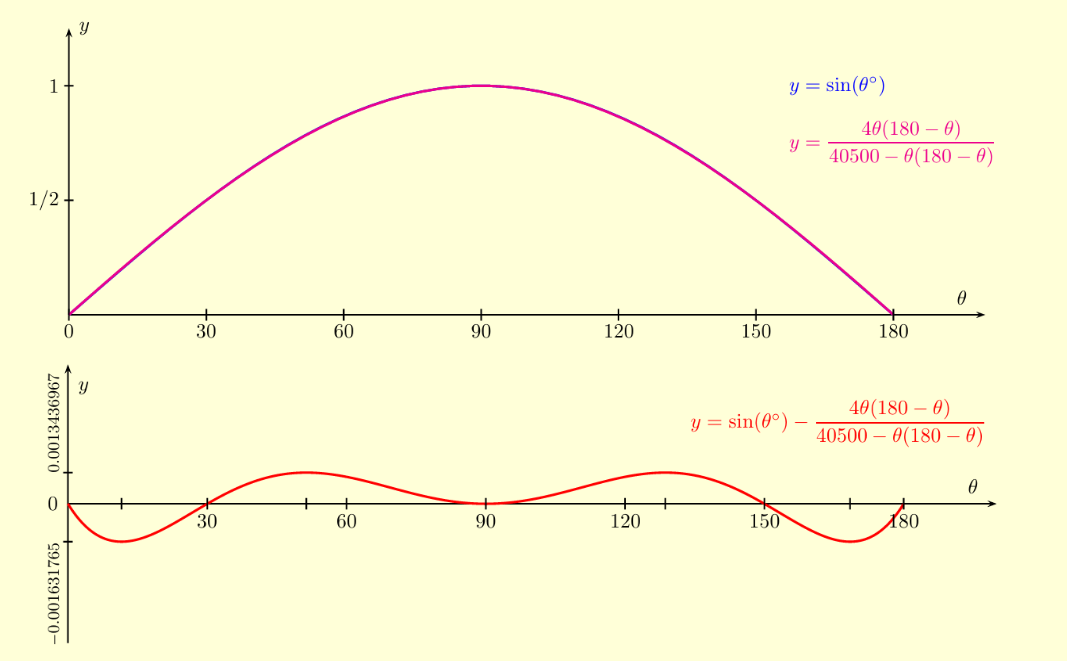
\includegraphics[width=0.7\linewidth]{bhaskara-final.png}
    \caption{Bhaskara's Approximation of Sin($\theta^{\circ}$)}
    \label{fig:sindegA2}
\end{figure}  

Now, with Bhaskara's approximation, we have sin(1$^{\circ}$) as $\frac{4(179)}{40500-179}$ = 0.01776, which is accurate to only 3 decimal places, and is in fact less accurate then the simple $\sin x \approx x$ approximation as seen in n = 1 of the Taylor series. So, Bhaskara's approximation in today's world is not of significant use; even a few terms from the Taylor series are more accurate - still, for his time, his approximation was fairly accurate and commendable.

\section{Method 2: Known Trig Ratios and De Moivre's} 

This method involves finding sin(15$^{\circ}$) and sin(15$^{\circ}$) geometrically, so with trigonometric identities sin(3$^{\circ}$) can be found, and with De Moivre's sin(1$^{\circ}$) can be exactly found.

\subsection{Deriving sin(18) and sin(15) with geometry}
To later find sin(3$^{\circ}$), it will be needed to first derive sin(18$^{\circ}$) and sin(15$^{\circ}$), from where we can get the cosines, and then use the angle difference formula.
\subsubsection{The 15-75-90 triangle}
Let us first take a 30-60-90 triangle, for which the ratios have been previously found, and use it to form a 15-75-90 triangle. Taking triangle ABC of side lengths 1, $\sqrt{3}$, and 2, we may then extend the $\sqrt{3}$ side by 2, as shown in Figure \ref{fig:15first}.\\

\begin{figure}[h]
    \centering
    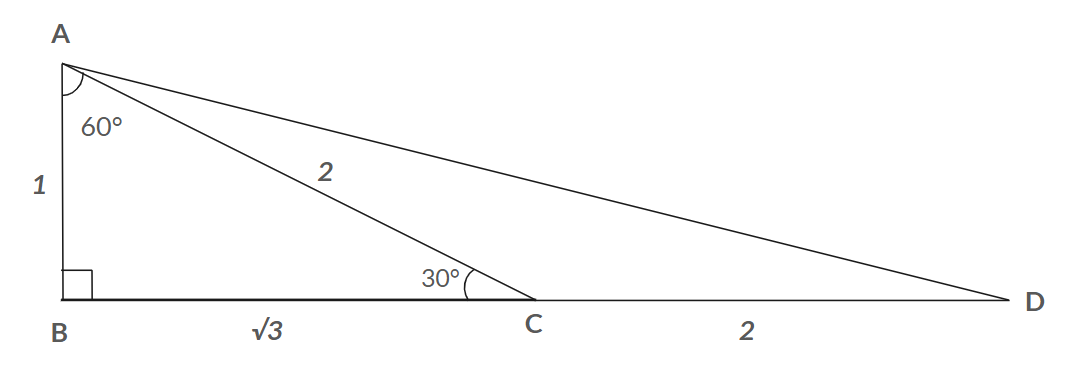
\includegraphics[width=0.8\linewidth]{15-75-90.png}
    \caption{Formation of a 15-75-90 Triangle}
    \label{fig:15first}
\end{figure}

Clearly, $\triangle$ACD is an isosceles triangle, meaning that $\measuredangle$CAD = $\measuredangle$ADC. Since $\measuredangle$ACD must equal $180-30 = 150^{\circ}$, we hence know that $\measuredangle$CAD = $\measuredangle$ADC = $15^{\circ}$. This clearly forms a 15-75-90 triangle, and we can now also use the Pythagoras Theorem to find that side AD is of length $\sqrt{(2+\sqrt{3})^2+1^2} = \sqrt{4+3+4\sqrt{3}+1} = \sqrt{8+4\sqrt{3}}$. Now, to further simplify this square root, we may assume that there is some $a$ and $b$ such that $(\sqrt{a}+\sqrt{b})^2=8+4\sqrt{3}$ . Expanding the left side, this means $a+b+2\sqrt{ab}=8+4\sqrt{3}$, or $a+b+2\sqrt{ab}=8+2\sqrt{12}$. Solving the system of $ab=12, a+b=8$, we have $b(8-b)=12 \rightarrow b^2 - 8b + 12 = 0 \rightarrow (b-6)(b-2) = 0$. As such, we know a and b are 6 and 2, meaning $\sqrt{8+4\sqrt{3}} = \sqrt{6}+\sqrt{2}$. We can hence show the completed triangle in Figure \ref{fig:15final}:

\begin{figure}[h]
    \centering
    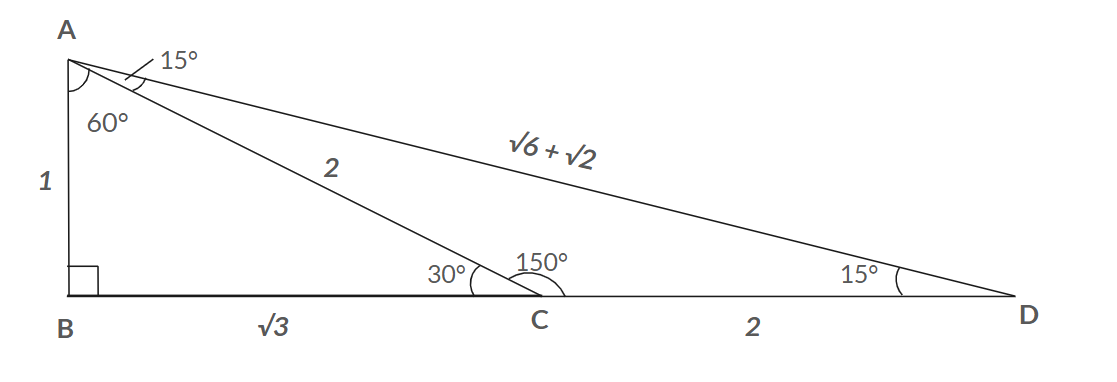
\includegraphics[width=0.8\linewidth]{15-75-90-complete.png}
    \caption{Complete 15-75-90 Triangle}
    \label{fig:15final}
\end{figure}

From our formed triangle, we may now find sin($15^{\circ}$) and rationalise, and also find cos($15^{\circ}$).

\[
    \sin(15^{\circ}) = \frac{1}{\sqrt{6}+\sqrt{2}} = \frac{\sqrt{6}-\sqrt{2}}{\sqrt{6}^2-\sqrt{2}^2}=\frac{\sqrt{6}-\sqrt{2}}{4}
\]
\[
    \cos(15^{\circ}) = \frac{2+\sqrt{3}}{\sqrt{6}+\sqrt{2}} = \frac{(2+\sqrt{3})(\sqrt{6}-\sqrt{2})}{4} = 
\]
\[
\frac{2\sqrt{6}-2\sqrt{2}+\sqrt{18}-\sqrt{6}}{4} =  \frac{\sqrt{6}-2\sqrt{2}+3\sqrt{2}}{4} = \frac{\sqrt{6}+\sqrt{2}}{4}
\]

\subsubsection{The 18-72-90 triangle}

To find sin($18^{\circ}$) geometrically, we can use the following isosceles 36-72-72 triangle ABD, where we can fix the lengths AB and AD to be 1, and let BD be $x$ which we want to find. Then, as shown in Figure \ref{fig:18tri1st}, we take the angle bisector of $\angle{ABD}$ to side AD, forming segment BC.

\begin{figure}[h]
    \centering
    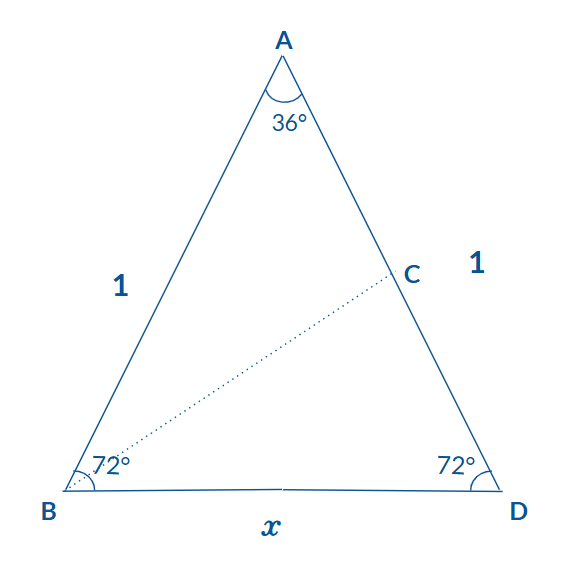
\includegraphics[width=0.5\linewidth]{18tri1st.png}
    \caption{Formation of a 36-72-72 Triangle}
    \label{fig:18tri1st}
\end{figure}

By bisecting $\angle{ABD}$, we in fact form $\triangle{CBD}$ in which $\measuredangle CBD = 36^{\circ}$ and  $\measuredangle CDB = 72^{\circ}$, meaning that $\measuredangle BCD = 72^{\circ}$ by triangle angle sum, and hence it is also isosceles, meaning that BC has length $x$. Further, as $\measuredangle ABC = 36^{\circ}$, $\triangle ABC$ is also isosceles, and the length of AC must be x, so CD has length $1-x$. Clearly, $\triangle CBD$ is similar to $\triangle ABD$ by Angle-Angle similarity, and as such, the side ratios are equal, so we know $\frac{x}{1-x}=\frac{1}{x}$. This forms the quadratic $x^2+x-1=0$, which by the quadratic formula yields that $x=\frac{-1\pm \sqrt{5}}{2}$, and as $x$ must be positive, $x=\frac{\sqrt{5}-1}{2}$. As shown in Figure \ref{fig:18comp}, this allows us to form an 18-72-90 triangle in which sin($15^{\circ}$) is evident.

\begin{figure}[h]
    \centering
    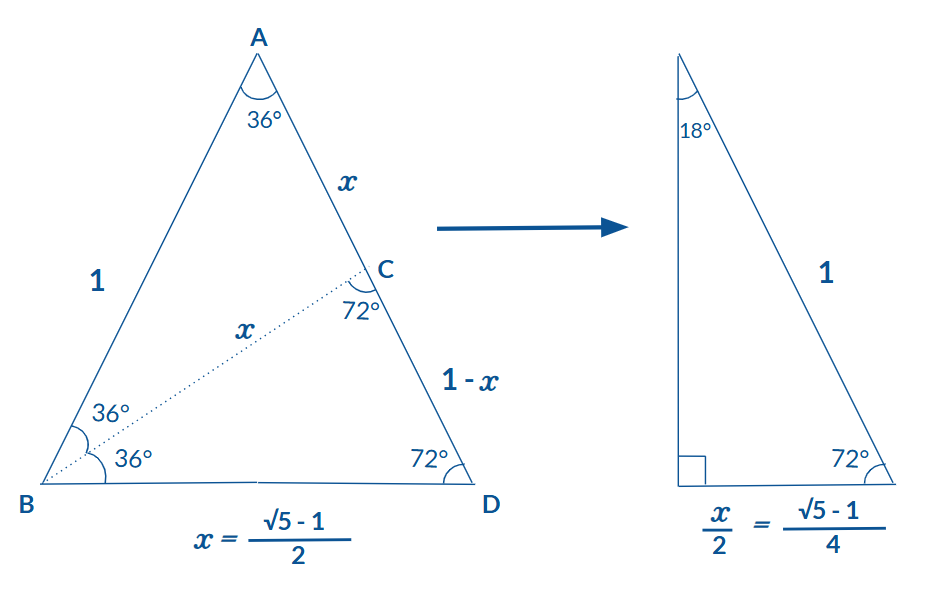
\includegraphics[width=0.8\linewidth]{18-72-90-complete.png}
    \caption{Complete Geometric Proof of sin(18$^{\circ}$)}
    \label{fig:18comp}
\end{figure}

By forming a triangle of 18-72-90 right from the isosceles triangle, we can take our value of $x$ divided by 2 to obtain the value of sin(18$^{\circ}$), which as per the diagram is $\frac{\sqrt{5}-1}{4}$. Using the Pythagoras trigonometric identity, we can also find that cos(18$^{\circ}$) = $\frac{\sqrt{10+2\sqrt{5}}}{4}$.

Now that the sines and cosines of 15$^{\circ}$ and 18$^{\circ}$ have been geometrically found, let us find sin(3$^{\circ}$) with a trigonometric identity.

\subsection{Using Angle Subtraction Formula to find sin(3)}
According to the International Baccalaureate Formula booklet,

\begin{center}
$\sin(A \pm B) = \sin A \cos B \pm \cos A \sin B$
\end{center}

Taking this as $\sin(18^{\circ} - 15^{\circ})$, we add the known values:

\[
\sin{3^{\circ}} = \left(\frac{\sqrt{5}-1}{4}\right)\left(\frac{\sqrt{6}+\sqrt{2}}{4}\right) - \left(\frac{\sqrt{10+2\sqrt{5}}}{4}\right)\left(\frac{\sqrt{6}-\sqrt{2}}{4}\right)
\]
Multiplying this out and combining we have:

\[
\sin{3^{\circ}} = \left(\frac{\sqrt{30}+\sqrt{10}-\sqrt{6}-\sqrt{2}}{16}\right) - \left(\frac{\sqrt{60+12\sqrt{5}}-\sqrt{20+4\sqrt{5}}}{16}\right)
\]
\[
 = \frac{\sqrt{30}+\sqrt{10}-\sqrt{6}-\sqrt{2}-2\sqrt{15+3\sqrt{5}}+2\sqrt{5+\sqrt{5}}}{16}
\]

To proceed, let us first notice that $\sqrt{15+3\sqrt{5}} = \sqrt{3}\sqrt{5+\sqrt{5}}$, and that this cannot be simplified further, so we can simply write our answer of $\sin{3^{\circ}}$ as:

\[
\sin{3^{\circ}} =  \frac{\sqrt{30}+\sqrt{10}-\sqrt{6}-\sqrt{2}-2(\sqrt{3}-1)\sqrt{5+\sqrt{5}}}{16}
\]

\subsection{De Moivre's Theorem to find sin(1$^{\circ}$)}
Now, the vital theorem called De Moivre's will allow us to use sin(3$^{\circ}$) in finding sin(1$^{\circ}$), though it will be seen that sin(1$^{\circ}$) cannot be written exactly with only real numbers.

Let's start by using De Moivre's to find a simplified expression for $\sin3\theta$. De Moivre's states that:

\[
\cos{n\theta} + i\sin{n\theta} = (\cos{\theta} + i\sin{\theta})^n
\]

Substituting n as 3, we have:

\[
\cos{3\theta} + i\sin{3\theta} = (\cos{\theta} + i\sin{\theta})^3
\]
Using $(a+b)^3=a^3+b^3+3ab^2+3a^2b$
\[
 = \cos^3{\theta} + i^3\sin^3{\theta} +3i^2\cos{\theta}\sin^2{\theta}+3i\cos^2{\theta}\sin{\theta}
\]
Simplifying:
\[
\cos{3\theta} + i\sin{3\theta} = (\cos^3{\theta} -3\cos{\theta}\sin^2{\theta}) + (- i\sin^3{\theta} + 3i\cos^2{\theta}\sin{\theta})
\]
Factoring out $i$ as we only want the imaginary part which yields $\sin{3\theta}$:
\[
\sin{3\theta} = 3\cos^2{\theta}\sin{\theta} - \sin^3{\theta}
\]
As $\cos^2{\theta} =1-\sin^2{\theta}$:
\[
\sin{3\theta} = 3(1-\sin^2{\theta})\sin{\theta} - \sin^3{\theta} = 3\sin{\theta}-3\sin^3{\theta}-\sin^3{\theta}=-4\sin^3{\theta}+3\sin{\theta}
\]
Now, to find $\sin{\theta}$, we may use Cardano's formula to give us the roots of a cubic of the form $x^3+px+q$.

\[
x = \sqrt[3]{-\frac{q}{2} + \sqrt{\left(\frac{q}{2}\right)^2 + \left(\frac{p}{3}\right)^3}} + \sqrt[3]{-\frac{q}{2} - \sqrt{\left(\frac{q}{2}\right)^2 + \left(\frac{p}{3}\right)^3}}
\]

Making our equation equivalent to 0, and then fitting this form, with $x=\sin{\theta}$, and $p=\frac{-3}{4}$, and $q=\frac{A}{4}$ where we let A = $\sin{3\theta}$:
\[
x^3+\frac{-3}{4}x+\frac{\sin{3\theta}}{4}=x^3+\frac{-3}{4}x+\frac{A}{4}
\]

Now, substituting in Cardano's:
\[
x = \sqrt[3]{-\frac{A}{8} + \sqrt{\left(\frac{A}{8}\right)^2 + \left(\frac{-1}{4}\right)^3}} + \sqrt[3]{-\frac{A}{8} - \sqrt{\left(\frac{A}{8}\right)^2 + \left(\frac{-1}{4}\right)^3}}
\]
Let us simplify this to yield an expression for $\sin{1^{\circ}}$, by later substituting $\sin{3^{\circ}}$ as A once this is further simplified:
\[
x = \sqrt[3]{-\frac{A}{8} + \sqrt{\frac{A^2}{64} - \frac{1}{64}}} + \sqrt[3]{-\frac{A}{8} - \sqrt{\frac{A^2}{64} - \frac{1}{64}}}
\]
Further simplifying:
\[
x = \sqrt[3]{-\frac{A}{8} + \frac{\sqrt{A^2-1}}{8}} + \sqrt[3]{-\frac{A}{8} - \frac{\sqrt{A^2-1}}{8}}
\]
And finally:
\[
x = \sqrt[3]{\frac{\sqrt{A^2-1}-A}{8}} + \sqrt[3]{\frac{-\sqrt{A^2-1}-A}{8}}
\]
Substituting our expression for $\sin{3^{\circ}}$ will make this cumbersome, so let use write our expression for now as $\frac{p-q}{16}$ where:
\[
p=\sqrt{30}+\sqrt{10}-\sqrt{6}-\sqrt{2},\;q=2(\sqrt{3}-1)\sqrt{5+\sqrt{5}}
\]

Substituting this as A:

\[ x = \sqrt[3]{\frac{\sqrt{\left(\frac{p-q}{16}\right)^2-1}-\frac{p-q}{16}}{8}} + \sqrt[3]{\frac{-\sqrt{\left(\frac{p-q}{16}\right)^2-1}-\frac{p-q}{16}}{8}} \]

Now we have:

\[ x = \sqrt[3]{\frac{\sqrt{p^2+q^2-2pq-256}+q-p}{128}} + \sqrt[3]{\frac{-\sqrt{p^2+q^2-2pq-256}+q-p}{128}} \]

Let us find a few of the terms involving p and q  before substituting:
\[ p^2 = -16\sqrt{5} - 8\sqrt{15} + 24\sqrt{3} + 48 \]
\[q^2 = 80 + 16\sqrt{5} - 40\sqrt{3} - 8\sqrt{15}\]
\[ p^2 + q^2 = -16\sqrt{15} - 16\sqrt{3} + 128 \]
\[ -2pq = -16\sqrt{10-2\sqrt{5}}\]
\[ q-p = 2 (\sqrt{3} - 1) \sqrt{5 + \sqrt{5}} - \sqrt{2} (1 + \sqrt{3}) (\sqrt{5} - 1) \]

As the square root is the same for both terms of Cardano's formula, let us simplify the terms inside it:

\[-16\sqrt{15} - 16\sqrt{3} + 128 -16\sqrt{10-2\sqrt{5}}-256\]
\[= -16(\sqrt{15} + \sqrt{3} - 8 +\sqrt{10-2\sqrt{5}}+16)\]
\[= -16(\sqrt{3}+\sqrt{15} + \sqrt{10-2\sqrt{5}}+8)\]

Finally, using this in the formula, we have:
\small\[ x = \sqrt[3]{\frac{4i\sqrt{\sqrt{3}+\sqrt{15} + \sqrt{10-2\sqrt{5}}+8}+2 (\sqrt{3} - 1) \sqrt{5 + \sqrt{5}} - \sqrt{2} (1 + \sqrt{3}) (\sqrt{5} - 1)}{128}}\]
\[+\sqrt[3]{\frac{-4i\sqrt{\sqrt{3}+\sqrt{15} + \sqrt{10-2\sqrt{5}}+8}+2 (\sqrt{3} - 1) \sqrt{5 + \sqrt{5}} - \sqrt{2} (1 + \sqrt{3}) (\sqrt{5} - 1)}{128}} \]
Now, there is one last thing that must be considered, which is that there are 3 cube roots and we cannot be sure which one to use without checking. By calculating, we find that the principal cube root is not actually correct, and that the cube root to be used for the first term involves the first cube root of unity, while the second term involves the second cube root of unity. So, the final exact value of sin(1$^{\circ}$) as per this method is:
\[(-1-i\sqrt{3})\sqrt[3]{\frac{4i\sqrt{\sqrt{3}+\sqrt{15} + \sqrt{10-2\sqrt{5}}+8}+2 (\sqrt{3} - 1) \sqrt{5 + \sqrt{5}} - \sqrt{2} (1 + \sqrt{3}) (\sqrt{5} - 1)}{1024}}\]
\[-(1-i\sqrt{3})\sqrt[3]{\frac{-4i\sqrt{\sqrt{3}+\sqrt{15} + \sqrt{10-2\sqrt{5}}+8}+2 (\sqrt{3} - 1) \sqrt{5 + \sqrt{5}} - \sqrt{2} (1 + \sqrt{3}) (\sqrt{5} - 1)}{1024}} \]

After checking with a calculator, this indeed results in the exact value of sine of 1 degree, and the imaginary terms cancel out.

\section{Method 3: The Unit Circle}
\subsection{The Unit Circle for Sine and Cosine And Roots of Unity}
As seen in Figure \ref{fig:uC}, the unit circle for sine and cosine can tell us the values of (cos, sin) for each angle measure from 0 to 360 degrees. This also has a deep connection to roots of unity, for which the 12th roots of unity are shown. Similarly, if the 360th roots of unity are found, the first one will actually if put in $\cos \theta + i\sin \theta$ form, tell us the value of sin(1 degree), as we can take the imaginary part!
\begin{figure}[h]
    \centering
    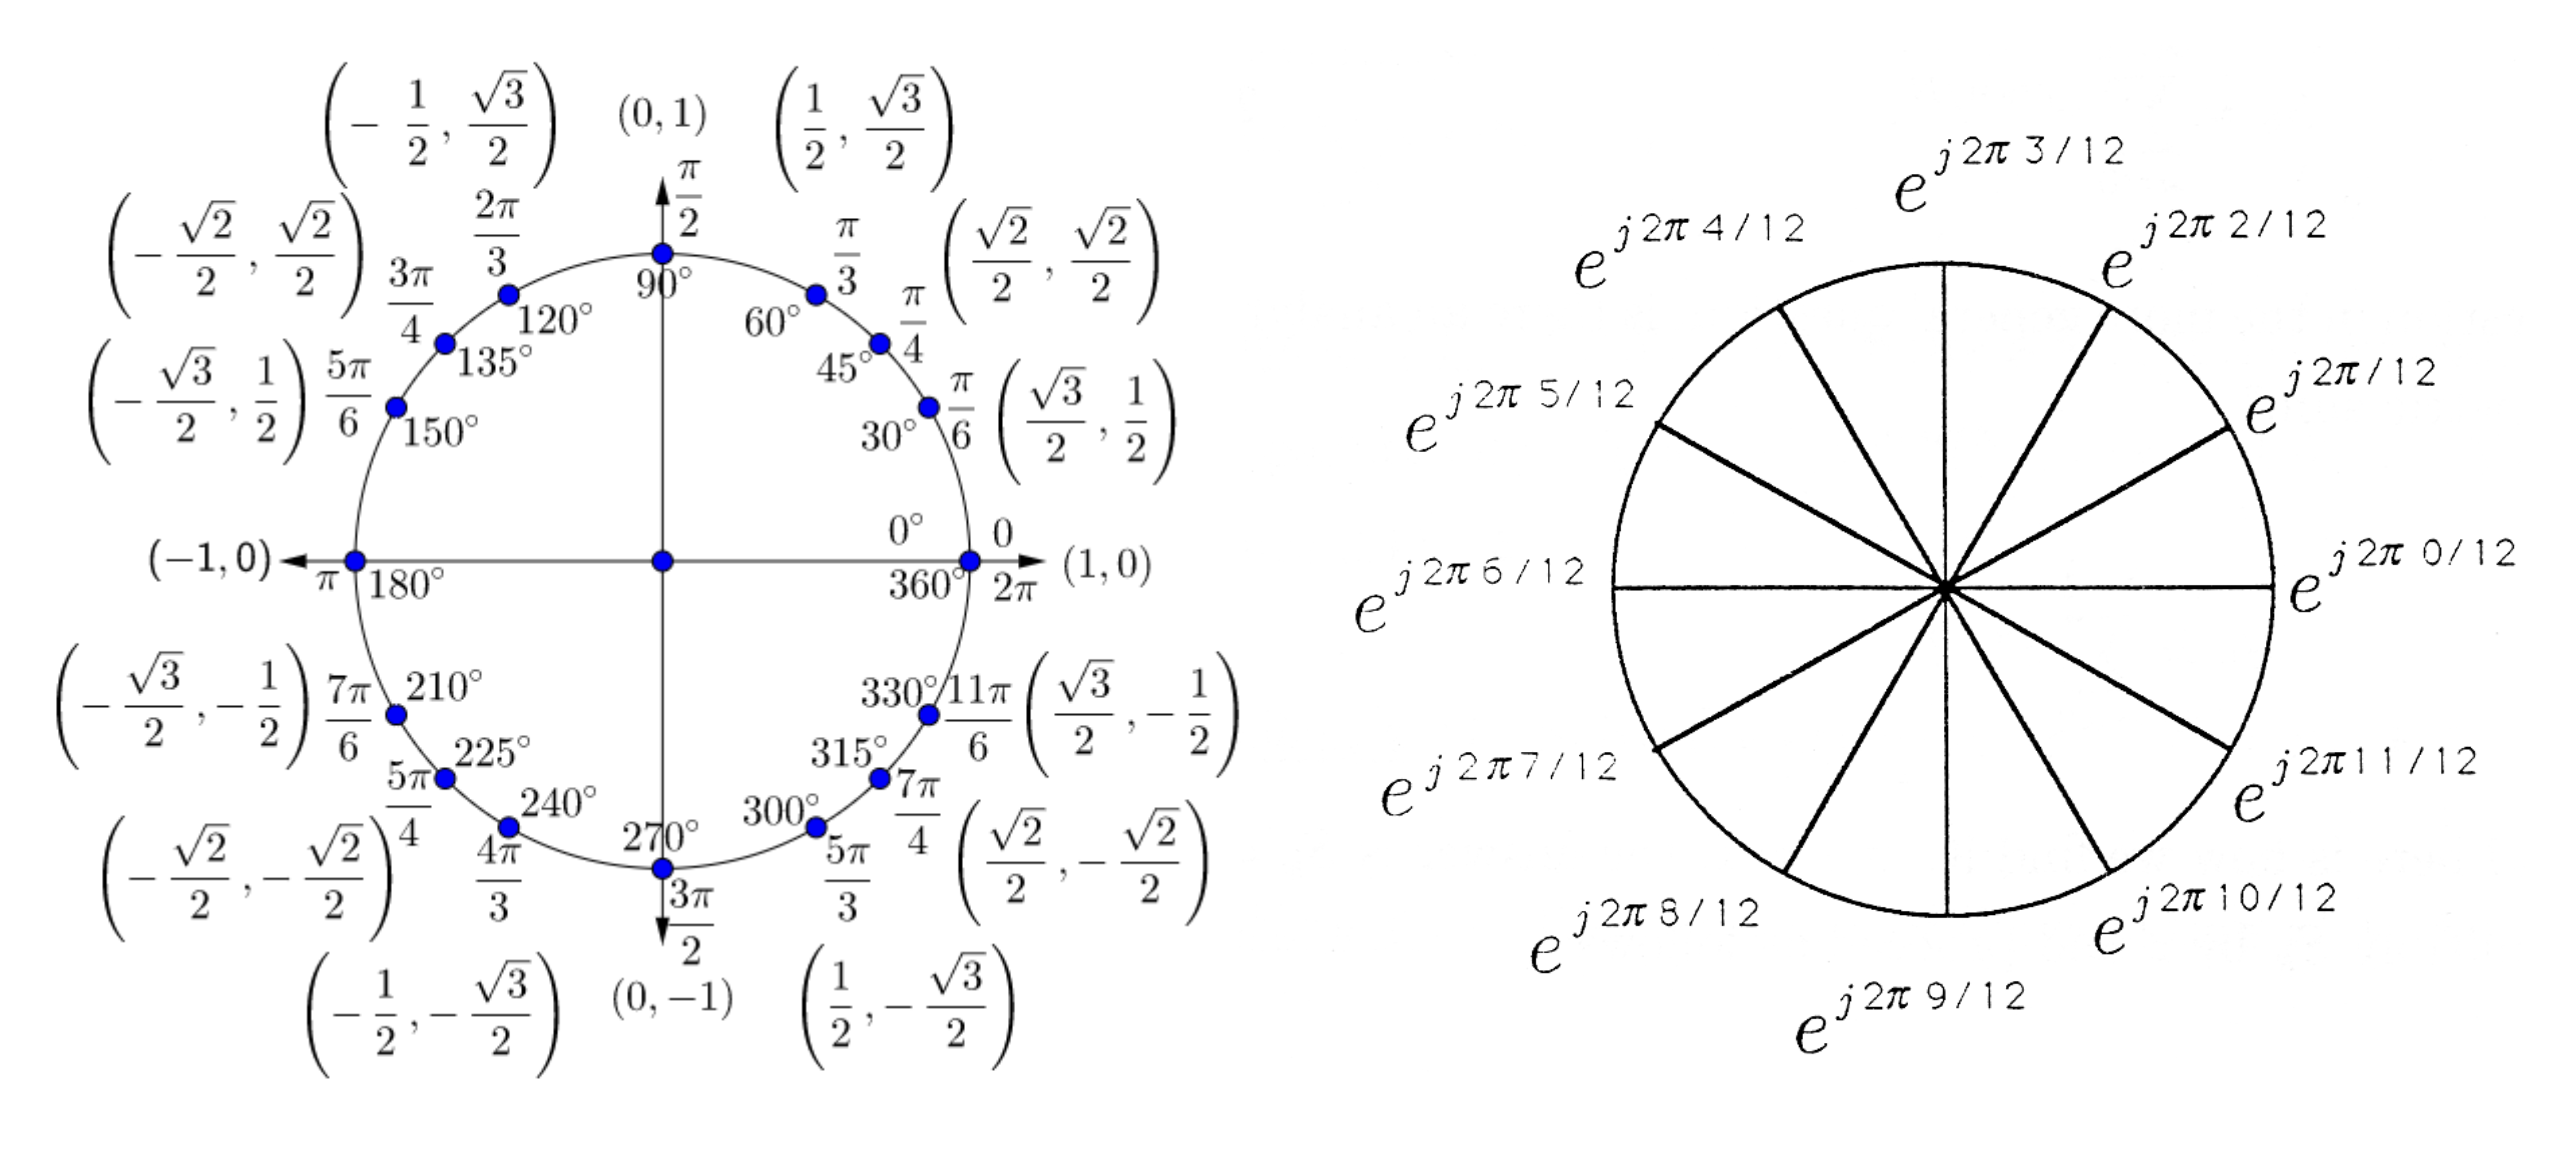
\includegraphics[width=0.9\linewidth]{unit-circle.png}
    \caption{The Unit Circle for Sine and Cosine, and Roots of Unity}
    \label{fig:uC}
\end{figure}

\subsection{The 360th root of unity to find sin(1)}
Let us first write the 360th root of unity as follows, where $k$ can be selected as any integer, due to the property of cosine and sine where 2$\pi$ added to $\theta$ does not change the value. As such, for 0,1,2,3...n-1 values of $k$, we will find distinct values of $z$, which will be seen for the 360th root of unity.
\[
z = (\cos{2k\pi} + i \sin{2k\pi})^{\frac{1}{n}}
\]
By De Moivre's, let us rewrite this as follows:
\[
z = \cos{\frac{2k\pi}{n}} + i \sin{\frac{2k\pi}{n}}
\]
Writing $z$ in Euler's form allows us to say:
\[
e^{\frac{2\pi ki}{n}} = \cos{\frac{2k\pi}{n}} + i \sin{\frac{2k\pi}{n}}
\]
Taking k as 1, as we want the first 360th root of unity, and n = 360:
\[
e^{\frac{\pi i}{180}} = \cos{\frac{\pi}{180}} + i \sin{\frac{\pi}{180}}
\]
Now we want to isolate sine. Let us first notice what happens when we take e to the power of $-\frac{\pi i}{180}$.
\[
e^{-\frac{\pi i}{180}} = \cos{\frac{-\pi}{180}} + i \sin{\frac{-\pi}{180}}
\]
As $\cos{-A}=\cos{A}$ and $\sin{-A}=-\sin{A}$, we have:
\[
e^{-\frac{\pi i}{180}} = \cos{\frac{\pi}{180}} - i \sin{\frac{\pi}{180}}
\]
So if we then take $e^{\frac{\pi i}{180}} - e^{-\frac{\pi i}{180}}$:
\[
e^{\frac{\pi i}{180}} - e^{-\frac{\pi i}{180}} = (\cos{\frac{\pi}{180}} + i \sin{\frac{\pi}{180}})-(\cos{\frac{\pi}{180}} - i \sin{\frac{\pi}{180}}) = 2i\sin{\frac{\pi}{180}}
\]
Hence,
\[
\sin{\frac{\pi}{180}} = \frac{e^{\frac{\pi i}{180}} - e^{-\frac{\pi i}{180}}}{2i}
\]
Which can be rewritten as:
\[
\sin{\frac{\pi}{180}} = \frac{(e^{i\frac{\pi}{2}})^{\frac{1}{90}} - (e^{-i\frac{\pi}{2}})^{\frac{1}{90}}}{2i}
\]
Now, with Euler's form we can say:
\[
e^{i\frac{\pi}{2}} = \cos{\frac{\pi}{2}} + i\sin{\frac{\pi}{2}} = i
\]
\[
e^{-i\frac{\pi}{2}} = \cos{\frac{-\pi}{2}} + i\sin{\frac{-\pi}{2}} = -i
\]
Substituting, we have:
\[
\sin{\frac{\pi}{180}} = \frac{i^{\frac{1}{90}} - (-i)^{\frac{1}{90}}}{2i}
\]
Now, here, $i$ can be replaced with $\pm \sqrt{-1}$, but for finding $\sin{1^{\circ}}$, we can take $\sqrt{-1}$, giving us the final formula:
\[
\sin{1^{\circ}} = \frac{\sqrt[90]{\sqrt{-1}} - \sqrt[90]{-\sqrt{-1}}}{2\sqrt{-1}}
\]
This is an interesting form of $\sin{1^{\circ}}$, as it stems from the imaginary realm yet comes out to be a simple formula one can type into a calculator. In fact, even the previous formula derived from Method 2 had imaginary numbers, and due to a special property that $\sin{1^{\circ}}$ is a \textit{transcendental} number, it cannot be written directly with only real numbers. 
\pagebreak
\section{Conclusion}
After comprehensively understanding various approximations of $\sin{1^{\circ}}$ and investigating two methods to find the exact value, that connect to concepts from complex numbers, geometry, algebra, and more, it is clear that for basic practical purposes, the approximation involving $\sin x = x$ is enough, and for more precise purposes, like engineering, a few terms of the Taylor series such as $x - \frac{x^3}{6} + \frac{x^5}{120}$ will be enough. 

However, for a deeper mathematical understanding, and from a theoretical perspective, the deep connections of $\sin{1^{\circ}}$ and the imaginary realm (such as roots of unity) should be understood, and the exact value found by Method 2, though it does not seem simple, can help in a generic understanding of number theory overall, as it is seen how the common looking $\sin{1^{\circ}}$ has the property of being a transcendental number, so it cannot be written as a purely real number. It also helps to see how from the geometrical, tangible real-world aspect of $\sin{18^{\circ}}$ and $\sin{15^{\circ}}$, one can dive into an algebraic approach with $\sin{3^{\circ}}$ and finally encounter imaginary numbers. 

In summary, the exploration of this IA into the sine ratio of 1 degree reveals the deep mathematical connection between trigonometry, algebra involving polynomials, calculus and power series, along with complex numbers; and it also clarifies why there are certain numbers, such as this sine ratio, that cannot be written as a simple algebraic expression with only real numbers. 
\pagebreak
\nocite{*}
\printbibliography

\end{document}
